\documentclass{article}
\usepackage[utf8]{inputenc} %кодировка
\usepackage[T2A]{fontenc}
\usepackage[english,russian]{babel} %русификатор 
\usepackage{mathtools} %библиотека матеши
\usepackage[left=1cm,right=1cm,top=2cm,bottom=2cm,bindingoffset=0cm]{geometry} %изменение отступов на листе
\usepackage{amsmath}
\usepackage{graphicx} %библиотека для графики и картинок
\graphicspath{}
\DeclareGraphicsExtensions{.pdf,.png,.jpg}
\usepackage{subcaption}
\usepackage{pgfplots}
\usepackage{listings}

\begin{document}
% НАЧАЛО ТИТУЛЬНОГО ЛИСТА
\begin{center}
    \Large
    Федеральное государственное автономное \\
    образовательное учреждение высшего образования \\ 
    «Научно-образовательная корпорация ИТМО»\\
    \vspace{0.5cm}
    \large
    Факультет программной инженерии и компьютерной техники \\
    Направление подготовки 09.03.04 Программная инженерия \\
    \vspace{1cm}
    \Large
    \textbf{Отчёт по лабораторной работе №1} \\
    По дисциплине «Вычислительная математика» (четвёртый семестр)\\
    \large
    \vspace{8cm}

    \begin{minipage}{.33\textwidth}
    \end{minipage}
    \hfill
    \begin{minipage}{.4\textwidth}
    
        \textbf{Студент}: \vspace{.1cm} \\
        \ Дениченко Александр P3212\\
        \textbf{Практик}:  \\
        \ Наумова Надежда Александровна
    \end{minipage}
    \vfill
Санкт-Петербург\\ 2024 г.
\end{center}

% КОНЕЦ ТИТУЛЬНОГО ЛИСТА 
\newpage
\begin{center}
    \LARGE
    \color{pink}
    \LaTeX \color{lime}.
\end{center}

\section{Цель работы}

Научиться искать решение СЛАУ при помощи численных методов, написать программу, которая будет совершать приближенные вычисления и находить решение, получая на вход матрицу из файла или консоли.


\section{Задание}
1. № варианта определяется как номер в списке группы согласно ИСУ.\\
2. В программе численный метод должен быть реализован в виде отдельной подпрограммы/метода/класса, в который исходные/выходные данные передаются в качестве параметров.\\
3. Размерность матрицы n<=20 (задается из файла или с клавиатуры - по выбору конечного пользователя).\\
4. Должна быть реализована возможность ввода коэффициентов матрицы, как с клавиатуры, так и из файла (по выбору конечного пользователя).\\
\\
Для прямых методов должно быть реализовано:

• Вычисление определителя

• Вывод треугольной матрицы (включая преобразованный столбец В)

• Вывод вектора неизвестных

• Вывод вектора невязок
\section{Блок-схема реализованного алгоритма}
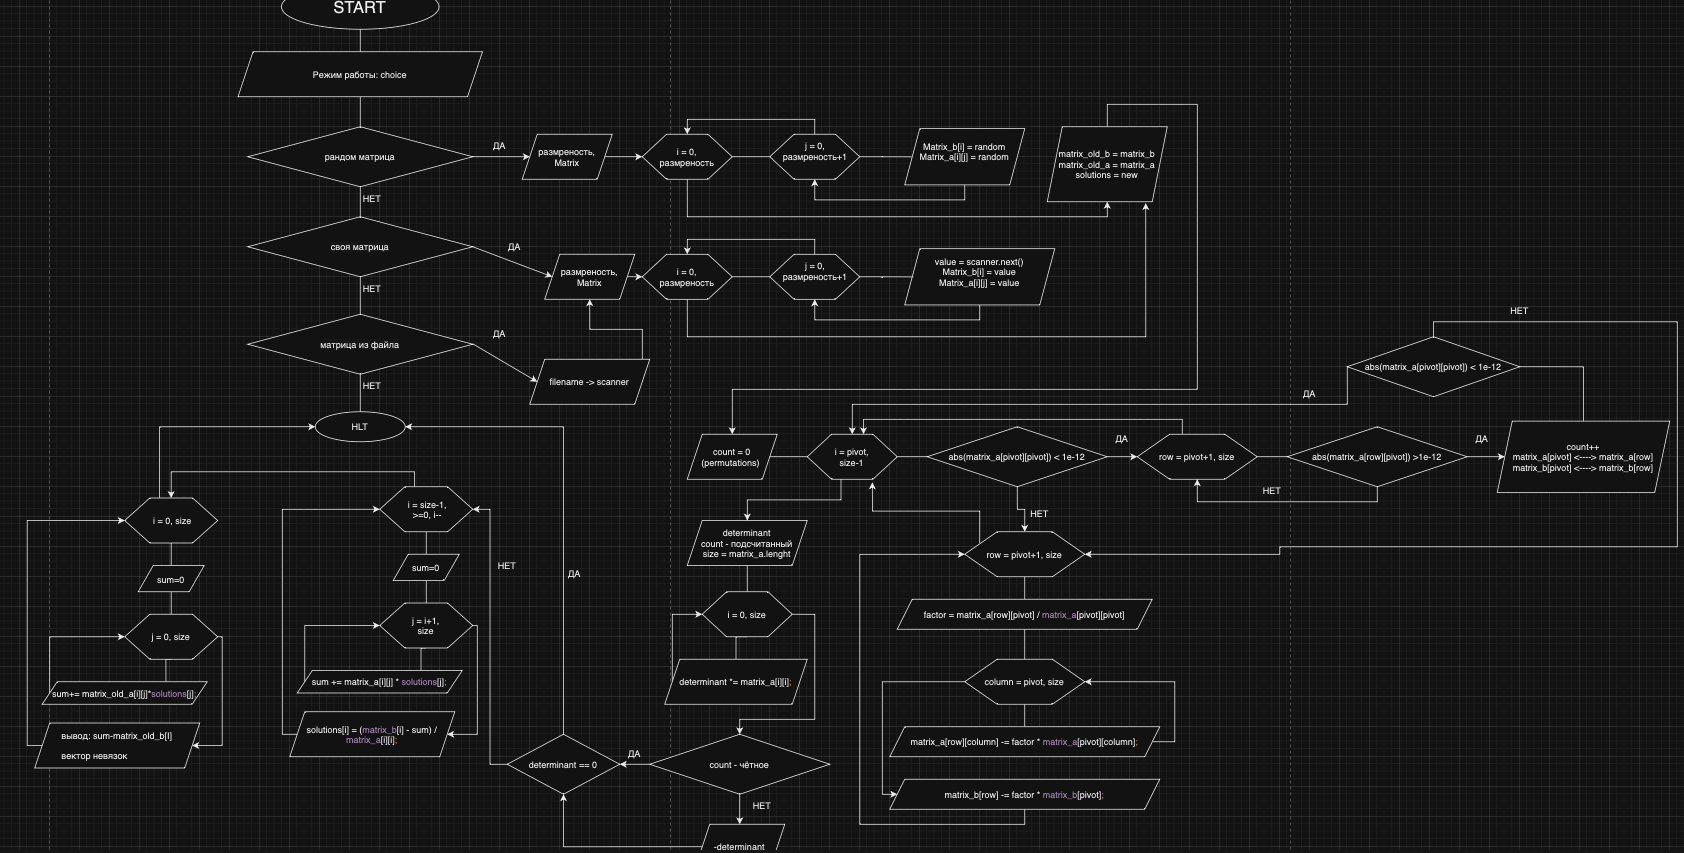
\includegraphics[width=1\textwidth]{2}
\section{Реализация (код) численного метода}
\textbf{Прямой ход:}
\begin{lstlisting}[frame=single, basicstyle=\ttfamily, breaklines=true, breakatwhitespace=true, postbreak=\mbox{\textcolor{red}{$\hookrightarrow$}\space}]
    public int gaussianElimination() {
        int count = 0;
        for (int pivot = 0; pivot < size - 1; pivot++) {
            if (Math.abs(matrix_a[pivot][pivot]) < 1e-12) {
                for (int row = pivot + 1; row < size; row++) {
                    if (Math.abs(matrix_a[row][pivot]) > 1e-12) {
                        count++;
                        double[] temp = matrix_a[pivot];
                        matrix_a[pivot] = matrix_a[row];
                        matrix_a[row] = temp;
                        double tempB = matrix_b[pivot];
                        matrix_b[pivot] = matrix_b[row];
                        matrix_b[row] = tempB;
                        break;
                    }
                }
            }
            if (Math.abs(matrix_a[pivot][pivot]) < 1e-12) {
                continue;
            }
            for (int row = pivot + 1; row < size; row++) {
                double factor = matrix_a[row][pivot] / matrix_a[pivot][pivot];
                for (int column = pivot; column < size; column++) {
                    matrix_a[row][column] -= factor * matrix_a[pivot][column];
                }
                matrix_b[row] -= factor * matrix_b[pivot];
            }
        }
        return count;
    }
\end{lstlisting}
\textbf{Обратный ход:}
\begin{lstlisting}[frame=single, basicstyle=\ttfamily, breaklines=true, breakatwhitespace=true, postbreak=\mbox{\textcolor{red}{$\hookrightarrow$}\space}]
    public void backwardSubstitution() {
        for (int i = size - 1; i >= 0; i--) {
            double sum = 0;
            for (int j = i + 1; j < size; j++) {
                sum += matrix_a[i][j] * solutions[j];
            }
            solutions[i] = (matrix_b[i] - sum) / matrix_a[i][i];
        }
    }
\end{lstlisting}
\section{Ссылка на GitHub с основной реализацией}
https://github.com/Alex-de-bug/cm\_math/tree/main/lab1
\section{Пример работы программы}
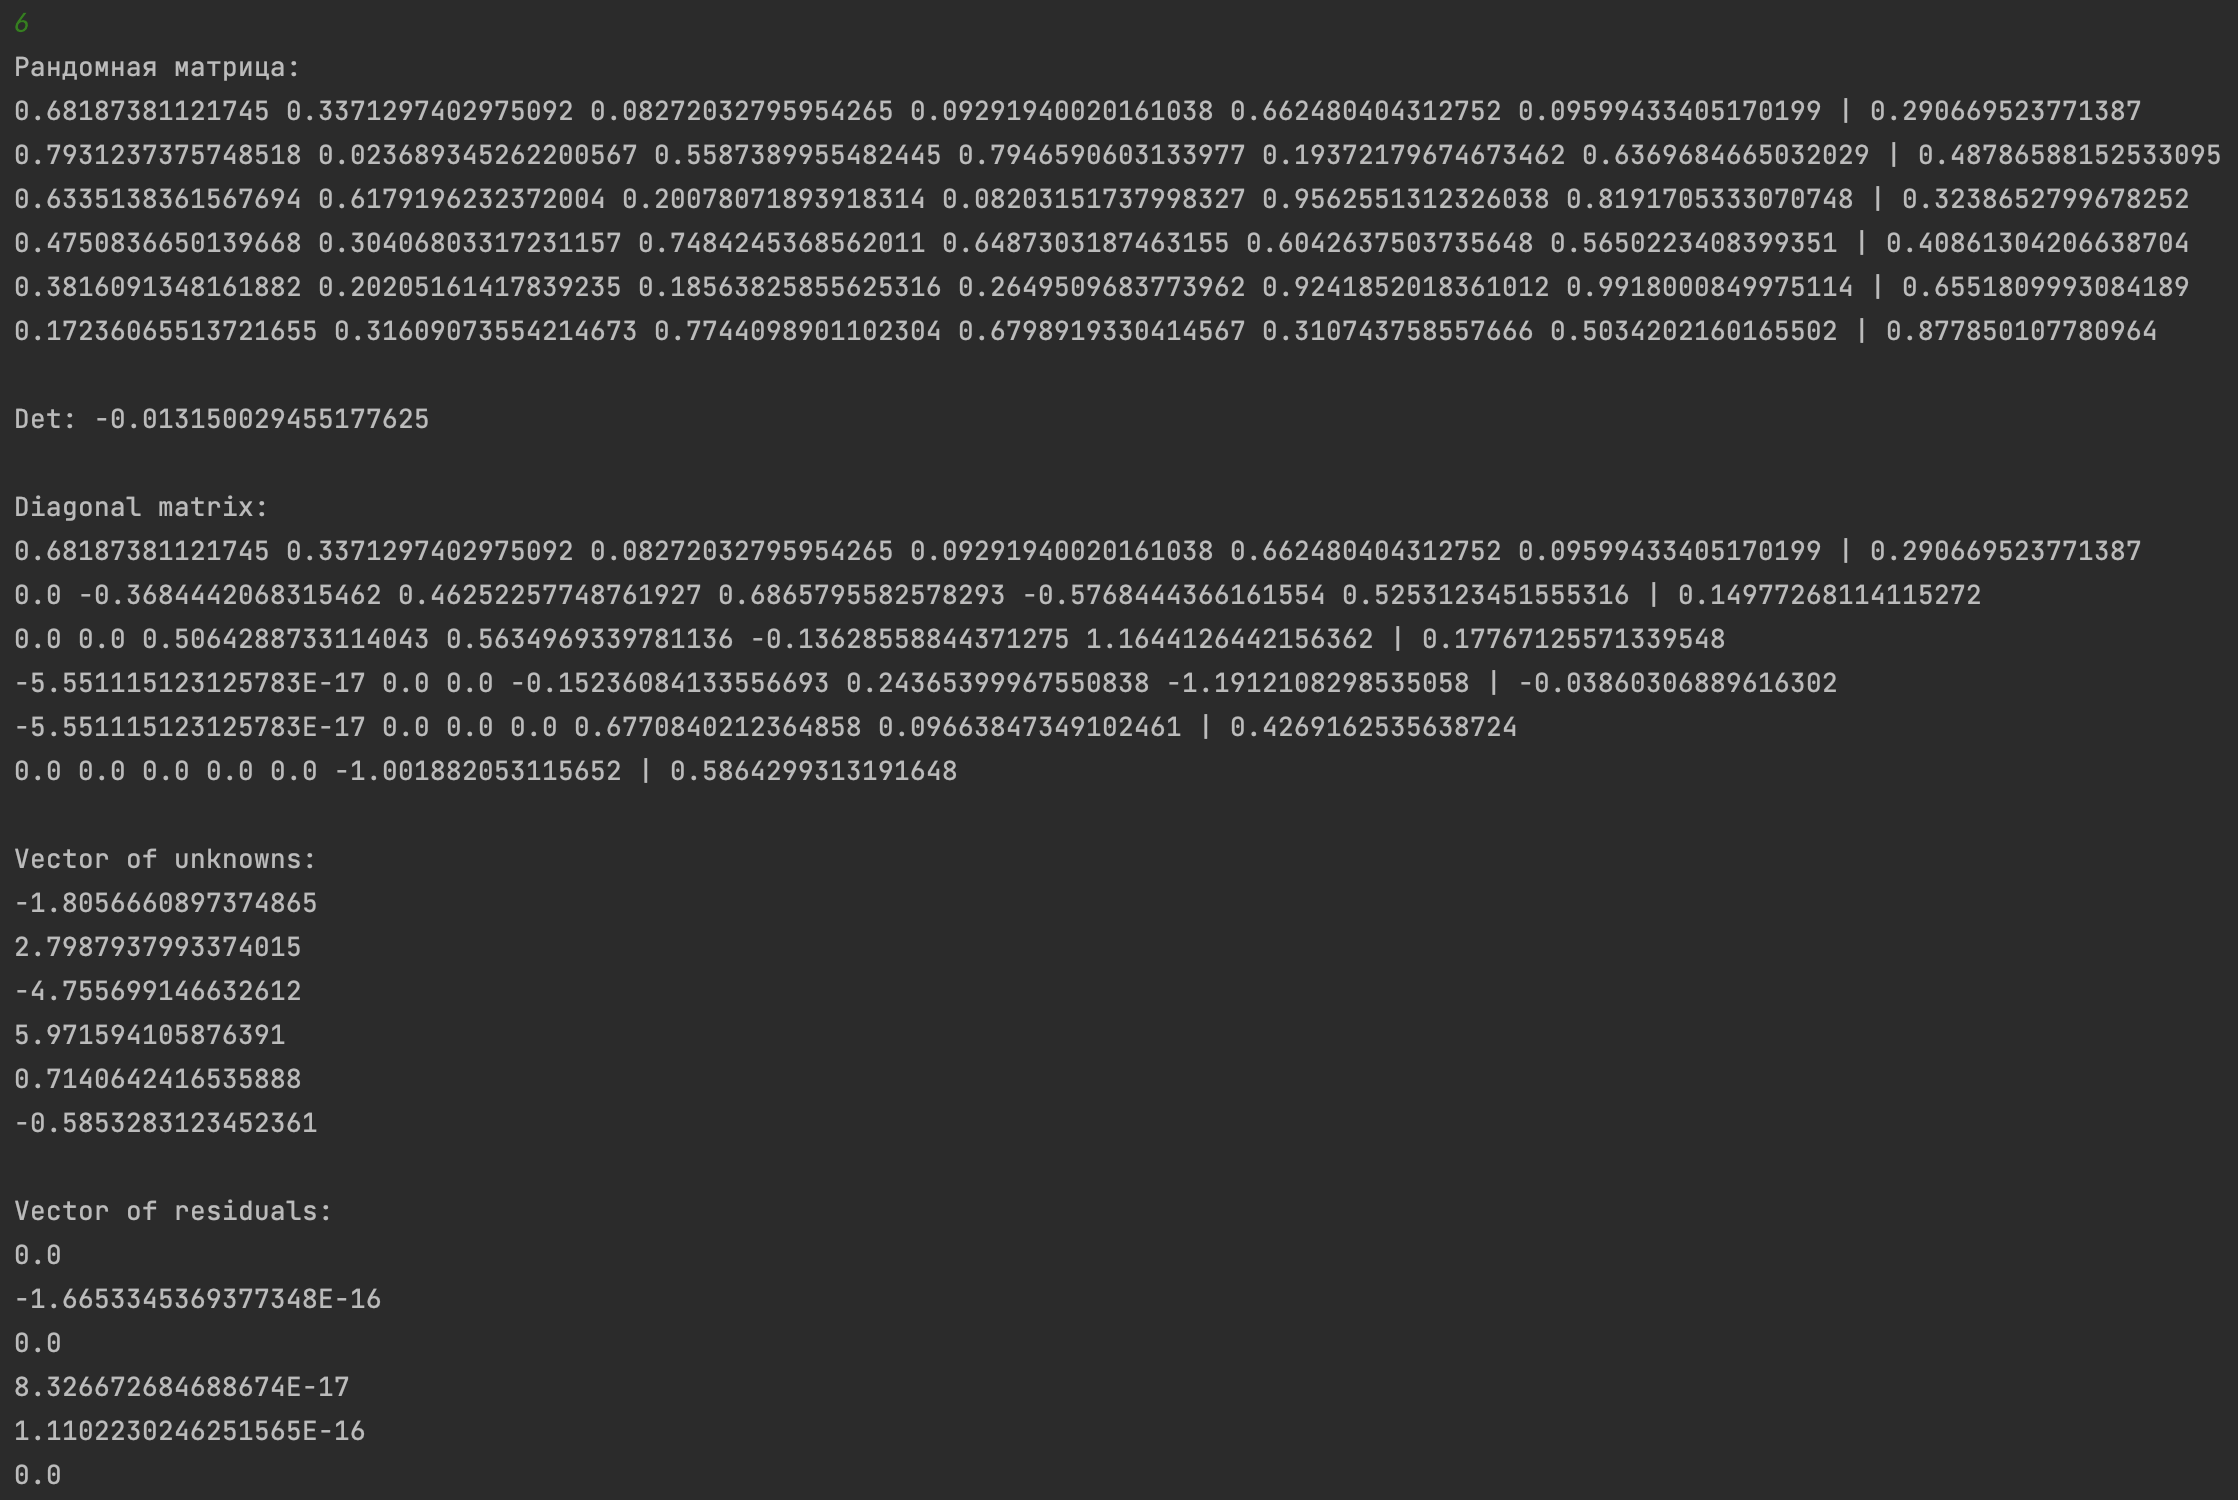
\includegraphics[width=1\textwidth]{3}
\section{Вывод}

Был изучен метод Гаусса для подсчёта СЛАУ. Получилось реализовать данный метод в ЯП Java. Это было великолепной практикой, я узнал по каким принципам работают сайты-решаторы.


\end{document}
